\chapter{Аналитический раздел}

\section{Выбор подхода к реализации драйвера на ОС Linux}

Одной из основных задач операционной системы является управление аппаратной частью. Ту программу или тот кусок программного кода, который предназначен для управления конкретным устройством, и называют обычно драйвером устройства. Необходимость драйверов устройств в операционной системе объясняется тем, что каждое отдельное устройство воспринимает только свой строго фиксированный набор специализированных команд, с помощью которых этим устройством можно управлять. Причем команды эти чаще всего предназначены для выполнения каких-то простых элементарных операций. Если бы каждое приложение вынуждено было использовать только эти команды, писать приложения было бы очень сложно, да и размер их был бы очень велик. Поэтому приложения обычно используют какие-то команды высокого уровня (типа <<записать файл на диск>>), а о преобразовании этих команд в управляющие последовательности для конкретного устройства заботится драйвер этого устройства. Поэтому каждое отдельное устройство, будь то дисковод, клавиатура или принтер, должно иметь свой программный драйвер, который выполняет роль транслятора или связующего звена между аппаратной частью устройства и программными приложениями, использующими это устройство. \cite{kostomin}

В Linux драйверы устройств бывают трех типов.

\subsection{Драйверы первого типа} являются частью программного кода ядра (встроены в ядро). Соответствующие устройства автоматически обнаруживаются системой и становятся доступны для приложений. Обычно таким образом обеспечивается поддержка тех устройств, которые необходимы для монтирования корневой файловой системы и запуска компьютера. Примерами таких устройств являются стандартный видеоконтроллер VGA, контроллеры IDE-дисков, материнская плата, последовательные и параллельные порты.

\subsection{Драйверы второго типа} представлены модулями ядра. Они оформлены в виде отдельных файлов и для их подключения (на этапе загрузки или впоследствии) необходимо выполнить отдельную команду подключения модуля, после чего будет обеспечено управление соответствующим устройством. Если необходимость в использовании устройства отпала, модуль можно выгрузить из памяти (отключить). Поэтому использование модулей обеспечивает большую гибкость, так как каждый такой драйвер может быть переконфигурирован без остановки системы. Модули часто используются для управления такими устройствами как SCSI-адаптеры, звуковые и сетевые карты.

\subsection{Драйверы третьего типа}
Для таких устройств программный код драйвера поделен между ядром и специальной утилитой, предназначенной для управления данным устройством. Например, для драйвера принтера ядро отвечает за взаимодействие с параллельным портом, а формирование управляющих сигналов для принтера осуществляет демон печати lpd, который использует для этого специальную программу-фильтр. Другие примеры драйверов этого типа — драйверы модемов и X-сервер (драйвер видеоадаптера).

\subsection{Взаимодейсвтие пользователя с устройством}
Но надо специально отметить, что во всех трех случаях непосредственное взаимодействие с устройством осуществляет ядро или какой-то модуль ядра. А пользовательские программы взаимодействуют с драйверами устройств через специальные файлы, расположенные в каталоге /dev и его подкаталогах. То есть взаимодействие прикладных программ с аппаратной частью компьютера в ОС Linux осуществляется по схеме ~\ref{image:scheme}.
 
\begin{figure}[h]
  \centering
  \includegraphics[scale=0.8]{scheme.png}
  \caption{Взаимодейсвтие пользователя с устройством}
  \label{image:scheme}
\end{figure}

Такая схема \ref{image:scheme} обеспечивает единый подход ко всем устройствам, которые с точки зрения приложений выглядят как обычные файлы.

\subsection{Динамическая загрузка драйверов}
За основу был взят подход динамической загрузки драйвера, который представляет собой загрузку при помощи отдельных модулей с расширением *.ko (объект ядра).

\subsection{Загружаемые модули}
Одной из хороших особенностей Linux является способность расширения функциональности ядра во время работы. Это означает, что вы можете добавить функциональность в ядро (и убрать её), когда система запущена и работает. Часть кода, которая может быть добавлена в ядро во время работы, называется модулем. Ядро Linux предлагает поддержку довольно большого числа типов (или классов) модулей, включая, но не ограничиваясь, драйверами устройств. Каждый модуль является подготовленным объектным кодом (не слинкованным для самостоятельной работы), который может быть динамически подключен в работающее ядро программой «insmod» и отключен программой «rmmod». \cite{ldd}

\subsection{Отличие между модулями ядра и приложениями}
Хотя большинство малых и средних приложений выполняют от начала до конца одну задачу, каждый модуль ядра просто регистрирует себя для того, чтобы обслуживать в будущем запросы, и его функция инициализации немедленно прекращается. Иными словами, задача функции инициализации модуля заключается в подготовке функций модуля для последующего вызова; это как будто модуль сказал: <<Вот я и вот что я могу делать>>. Функция выхода модуля  вызывается только непосредственно перед выгрузкой модуля. Она сообщает ядру: <<Меня больше нет>>. Такой подход к программированию подобен программируемой обработке событий, но пока не все приложения управляются событиями, как модули ядра. Другое сильное отличие между событийно - управляемым приложением и кодом ядра в функции выхода: в то время как приложение, которое прекращает работу, может быть ленивым при высвобождении ресурсов или избегать очистки всего, функция выхода модуля должна тщательно отменить все изменения, сделанные функцией инициализации, или эти куски останутся вокруг до перезагрузки системы. 
Возможность выгрузить модуль является одной из тех особенностей подхода модуляризации, потому что это помогает сократить время разработки; можно тестировать последовательные версии новых драйверов, не прибегая каждый раз к длительному циклу выключения/перезагрузки. 
Приложение может вызывать функции, которые не определены: стадия линковки разрешает (определяет) внешние ссылки, используя соответствующие библиотечные функции. Printf является одной из таких вызываемых функций и определена в libc. Модуль, с другой стороны, связан только с ядром и может вызывать только те функции, которые экспортированы ядром, нет библиотек для установления связи. Например, функция printk, является версией printf, определённой в ядре и экспортированной для модулей. Она ведёт себя аналогично оригинальной функции с небольшими отличиями, главным из которых является отсутствие поддержки плавающей точки. Рисунок~\ref{image:module_in_kernel} показывает, как используются в модуле вызовы функций и указатели на функции, чтобы добавить ядру новую функциональность. \cite{ldd}

\begin{figure}[h]
  \centering
  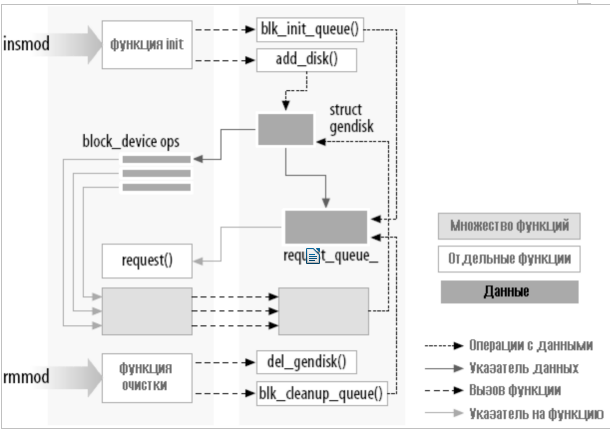
\includegraphics[scale=1]{module_in_kernel.png}
  \caption{Связи модуля в ядре}
  \label{image:module_in_kernel}
\end{figure}

Файлы исходников никогда не должны подключать обычные заголовочные файлы, потому что нет библиотеки, связанной с модулями, и очень специальные ситуации будут только исключениями. Только функции, которые фактически являются частью самого ядра, могут быть использованы в модулях ядра. Всё относящееся к ядру объявлено в заголовках, находящихся в дереве исходных текстов ядра; наиболее часто используемые заголовки живут в include/linux и include/asm, но есть и другие подкаталоги в папке include для содержания материалов, связанных со специфичными подсистемами ядра. 
Ещё одно важное различие между программированием ядра и прикладным программированием в том, как каждое окружение обрабатывает ошибки: в то время, как ошибка сегментации является безвредной при разработке приложений и всегда можно использовать отладчик для поиска ошибки в исходнике, ошибка ядра убивает по крайней мере текущий процесс, если не всю систему.

\subsection{Пространство пользователя и пространство ядра}
Модули работают в пространстве ядра, в то время как приложения работают в пользовательском пространстве. Это базовая концепция теории операционных систем.

На практике ролью операционной системы является обеспечение программ надёжным доступом к аппаратной части компьютера. Кроме того, операционная система должна обеспечивать независимую работу программ и защиту от несанкционированного доступа к ресурсам. Решение этих нетривиальных задач становится возможным, только если процессор обеспечивает защиту системного программного обеспечения от прикладных программ. 

Каждый современный процессор позволяет реализовать такое поведение. Выбранный подход заключается в обеспечении разных режимов работы (или уровней) в самом центральном процессоре. Уровни играют разные роли и некоторые операции на более низких уровнях не допускаются; программный код может переключить один уровень на другой только ограниченным числом способов. Unix системы разработаны для использования этой аппаратной функции с помощью двух таких уровней. Все современные процессоры имеют не менее двух уровней защиты, а некоторые, например семейство x86, имеют больше уровней; когда существует несколько уровней, используются самый высокий и самый низкий уровни. Под Unix ядро выполняется на самом высоком уровне (также называемым режимом супервизора), где разрешено всё, а приложения выполняются на самом низком уровне (так называемом пользовательском режиме), в котором процессор регулирует прямой доступ к оборудованию и несанкционированный доступ к памяти.
Unix выполняет переход из пользовательского пространства в пространство ядра, когда приложение делает системный вызов или приостанавливается аппаратным прерыванием. Код ядра, выполняя системный вызов, работает в контексте процесса - он действует от имени вызывающего процесса и в состоянии получить данные в адресном пространстве процесса. Код, который обрабатывает прерывания, с другой стороны, является асинхронным по отношению к процессам и не связан с каким-либо определённым процессом. 

Ролью модуля является расширение функциональности ядра; код модулей выполняется в пространстве ядра. Обычно драйвер выполняет обе задачи, изложенные ранее: некоторые функции в модуле выполняются как часть системных вызовов, а некоторые из них отвечают за обработку прерываний.
